\documentclass[a4paper,12pt,reqno]{amsart}
\usepackage{graphicx}
\usepackage{macros_M53}

% pour voir les solutions il faut enlever le commentaire de la ligne suivante
% \solutionstrue

\begin{document}

% ==================================
\hautdepage{

\ifsolutions{Solutions de l'examen de rattrapage}\else{Examen de rattrapage}\fi\par\normalfont\normalsize
8 juin 2016\\{[ durée: 3 heures ]}\par
}
% ==================================
\ifsolutions\else
% {\fontencoding{U}\fontfamily{futs}\selectfont\char 66\relax}
\tikz[baseline=(e.base)]{\NoAutoSpacing\node(e){!};\draw[red,ultra thick,line join=round,yshift=-.15ex](90:1em)--(210:1em)--(330:1em)--cycle;}
\textbf{Documents autorisés :}\textit{Une feuille A4 recto-verso écrite à la main.}

\tsvp

\vspace{7mm}
\fi

%-----------------------------------
\begin{exo} (Sous-espaces affines)
  \begin{enumerate}
    \item Démontrer la proposition du cours :

    \framebox{
      \parbox{\textwidth-3cm}{\vspace{1mm}
        \emph{
          Soient $\ev{E}$ et $\ev{F}$ deux espaces vectoriels, et $\vv\phi \in \lin(\ev{E},\ev{F})$ une application linéaire.
          Pour tout $\vv{v}\in\im\vv\phi\subset\ev{F}$, l'image réciproque $\vv\phi^{-1}(\vv{v})$ est un sous-espace affine de $\ev{E}$ de direction $\ker{\vv\phi}$.
        }
      }
    }

    \smallskip

    \item Soit $\mathcal{C}(\mathbb{R})$ l'espace vectoriel des fonctions continues sur $\mathbb{R}$. Montrer que $\ens{H} = \{ f \in \mathcal{C}(\mathbb{R}) : f(x-1)=f(x)+2, \ \forall x \in \mathbb{R} \}$
  est un sous-espace affine de $\mathcal{C}(\mathbb{R})$ . Déterminer
  un point de $\ens{H}$ et sa direction.

    \item Est-ce que le sous-ensemble de $\mathbb{R}^{2}$ d'équation $\{(x-1)^{2}+(x-y)^{2}=0\}$ est un sous-espace vectoriel et/ou un sous-espace affine ? Justifier votre réponse.
  \end{enumerate}
\end{exo}

\begin{solution}

  \begin{enumerate}
    \item Comme $\vv\phi$ est linéaire, $\ker{\vv\phi}$ est un sous-espace vectoriel. Soit $\vv{v}\in\im\vv\phi$, et $\vv{u}\in\ev{E}$ tel que $\vv\phi(\vv{u})=\vv{v}$. Soit $\vv{w} \in \ev{E}$, alors $\vv{u}+\vv{w} \in \vv\phi^{-1}(\vv{v})$ $\Leftrightarrow$ $\vv\phi(\vv{u}+\vv{w})=\vv{v}$ $\Leftrightarrow$ $\vv\phi(\vv{u})+\vv\phi(\vv{w})=\vv{v}$ $\Leftrightarrow$ $\vv\phi(\vv{w})=\vv{0}$, et donc $\vv\phi^{-1}(\vv{v}) = \vv{u} + \ker{\vv\phi}$. On vient de démontrer que $\vv\phi^{-1}(\vv{v})$ est un sous-espace affine de $\ev{E}$ de direction $\ker{\vv\phi}$.
    \item On note $\ev{P} = \{ f \in \mathcal{C}(\mathbb{R}) : f(x-1)=f(x), \ \forall x \in \mathbb{R} \}$ le sous-espace vectoriel des fonctions continues et $1$-périodiques. Soit $g(x)=-2x$, comme $g(x-1)=-2(x-1)=g(x)+2$, alors $g\in\ens{H}$. Soit $\phi \in \mathcal{C}(\mathbb{R})$, alors $g+\phi \in \ens{H}$ $\Leftrightarrow$ $\forall x \in \mathbb{R}, g(x-1)+\phi(x-1)=g(x)+\phi(x)+2$ $\Leftrightarrow$ $\forall x \in \mathbb{R}, \phi(x-1)=\phi(x)$ $\Leftrightarrow$ $\phi \in \ev{P}$. Ainsi on vient de démontrer que $\ens{H}=g+\ev{P}$ et donc $\ens{H}$ est un sous-espace affine de $\mathcal{C}(\mathbb{R})$ contenant le point $g$ et de direction $\ev{P}$.
    \item L'ensemble $\{(x-1)^{2}+(x-y)^{2}=0\}=\{(1,1)\}$ est un sous-espace affine de $\mathbb{R}^{2}$ de dimension $0$, car tout ensemble à un élément en est un. Mais il n'est pas un sous-espace vectoriel car $(0,0) \notin \{(1,1)\}$.
  \end{enumerate}
\end{solution}


%-----------------------------------
\begin{exo} (Géométrie dans $\mathbb{R}^{3}$)

  On se place dans l'espace affine euclidien $\mathbb{R}^{3}$.

  \begin{enumerate}

    \item On considère les deux matrices
    \[
      \renewcommand{\arraystretch}{.77}
      \frac{1}{3}
      \begin{pmatrix}
        -1 & 2 & -2 \\
         2 &-1 & -2 \\
        -2 &-2 & -1
      \end{pmatrix}
      \qquad\text{et}\qquad
      \begin{pmatrix}
        -1 & 2 & -2 \\
         2 &-1 & -2 \\
        -2 &-2 & -1
      \end{pmatrix}
    .\]

    Laquelle de ces deux matrices est la matrice d'une isométrie de $\mathbb{R}^{3}$ ?
  \end{enumerate}

    \emph{Pour la suite de l'exercice on note $M$ cette matrice de $O(\mathbb{R}^{3})$, ainsi que l'application linéaire qu'elle définit.}

  \begin{enumerate}[resume]

    \item Décrire $M$ en détail (nature, points fixes, paramètres).

    \item Soit $T_{\vv{v}}$ la translation de vecteur $\vv{v} = (1,0,1)$. Quelle est la nature de l'application composée $T_{\vv{v}}M$ ?

    \item Soit $S$ la symétrie orthogonale par rapport au plan d'équation $\{x+y-z=1\}$. Quelle est la nature de l'application composée $MS$ ?
  \end{enumerate}
\end{exo}

\begin{solution}
  % walfram alpha : {{-1,2,-2},{2,-1,-2},{-2,-2,-1}}/3
  % octave : M = [-1 2 -2 ; 2 -1 -2 ; -2 -2 -1]/3

  % Les espaces propres de $M$ sont $E_{1}=\affspan{(1,1,-1)}$ et $E_{-1}=\affspan{(1,0,1),(-1,1,0)}$.
  % Le polynomé charactéristique est $x^{3}+x^{2}-x-1$.

  \begin{enumerate}
    \item Les vecteurs colonnes des deux matrices forment une base orthogonale, mais seulement ceux de la première forment une b.o.n. (ceux de la deuxième sont de norme $9$). Donc la matrice orthogonale $M$ est la première.
    \item Comme $\det(M)=1$, $M$ est une rotation. Pour trouver l'axe de rotation on cherche l'ensemble des vecteurs fixes : $\ker(M-I)$, et on trouve $E_{1}=\affspan{(1,1,-1)}$. Soit $\theta$ l'angle de rotation. Comme $2\cos(\theta)+1=\tr(M)=-1$ on trouve que $\theta=\pi$. Ainsi $M$ est une rotation d'angle $\pi$ autour de l'axe $\affspan{(1,1,-1)}$, autrement dit c'est une symétrie axiale d'axe $\affspan{(1,1,-1)}$.
    \item Comme $\vv{v} \perp (1,1,-1)$, d'après le cours, $T_{\vv{v}}M$ est aussi une symétrie axiale.
    \item Comme $\{x+y-z=1\}$ est perpendiculaire à $\affspan{(1,1,-1)}$, la composé $MS$ est une symétrie centrale de centre $\{x+y-z=1\} \cap \affspan{(1,1,-1)} = {(\frac13,\frac13,-\frac13)}$. En réalité dans une base orthonormée $(\vv{e}_{1}, \vv{e}_{2}, \vv{e}_{3})$ avec $\vv{e}_{1}=\frac{1}{\sqrt{3}}(1,1,-1)$ nous avons les parties linéaires qui sont $\vv{M}=\begin{psmallmatrix}1&0&0\\0&-1&0\\0&0&-1\end{psmallmatrix}$, $\vv{S}=\begin{psmallmatrix}-1&0&0\\0&1&0\\0&0&1\end{psmallmatrix}$, et donc $\vv{MS}=-\id$.
  \end{enumerate}
\end{solution}


%-----------------------------------
\begin{exo} (Construction d'une ellipse)

  \begin{wrapfigure}{r}{57mm}
    \centering\vspace{-7mm}
    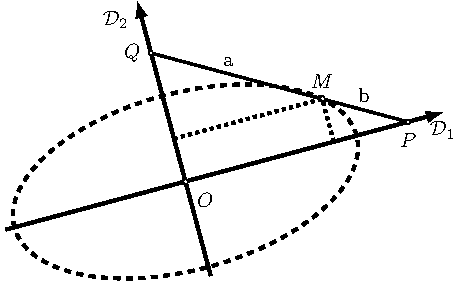
\includegraphics[width=57mm]{img_ellipse_segment}
  \end{wrapfigure}
  Soient deux droites $\ens{D}_{1}$ et $\ens{D}_{2}$ orthogonales qui se coupent en un point $O$. Soient deux nombres positifs $a,b>0$. Pour toute paire de points $(P,Q)$ telle que $P \in \ens{D}_{1}$, $Q \in \ens{D}_{2}$ et $\d(P,Q)=a+b$ on considère le point $M=\frac{a}{a+b}P+\frac{b}{a+b}Q$.

  Montrer que le lieu des points $M$ est une ellipse.

\end{exo}

\begin{solution}

  On se place dans un repère orthonormé de centre $O$ et d'axes $\ens{D}_{1}$ et $\ens{D}_{2}$. Nous allons démontrer que le lieu des points $M$ est l'ellipse $\ens{E}=\left\{(x,y)\ \big|\ \left(\frac{x}{a}\right)^{2} + \left(\frac{y}{b}\right)^{2} = 1 \right\}$.

  Soit $M$ comme dans l'énoncé, ayant $(x,y)$ pour coordonnées dans le repère fixé. D'après Thalès $|OP|=|x|\frac{a+b}{a}$ et $|OQ|=|y|\frac{a+b}{b}$. Et comme $|OP|^{2}+|OQ|^{2}=|PQ|^{2}$ (d'après Pythagore), on trouve $\left(x\frac{a+b}{a}\right)^{2}+\left(y\frac{a+b}{b}\right)^{2} = (a+b)^{2}$ $\Leftrightarrow$ $\left(\frac{x}{a}\right)^{2}+\left(\frac{y}{b}\right)^{2} = 1$. Et donc $M \in \ens{E}$.

  Réciproquement, soit $M \in \ens{E}$ ayant $(x,y)$ pour coordonnées dans le repère fixé.
  On pose $P = (x\frac{a+b}{a}, 0)$ et $Q = (0, y\frac{a+b}{b})$. Alors $\frac{a}{a+b}P+\frac{a}{a+b}Q = (x,y) = M$. Pour finir on observe que $|PQ|^{2}=\left(x\frac{a+b}{a}\right)^{2}+\left(y\frac{a+b}{b}\right)^{2} = (a+b)^{2}\left[\left(\frac{x}{a}\right)^{2} + \left(\frac{y}{b}\right)^{2}\right] = (a+b)^{2}$ et donc $|PQ|=a+b$.

\end{solution}


%-----------------------------------
\begin{exo} (Géométrie dans le plan complexe)

  \begin{minipage}{.7\linewidth}\smallskip
    On se place dans le plan euclidien identifié avec $\mathbb{C}$. Soit $z \in \mathbb{C}$ avec $\im(z)>0$. Soient $A$, $B$ et $D$ trois points d'affixes respectives $0$, $1$ et $z$. Soit un quatrième point $C$ tel que $A,B,C,D$ forment un parallélogramme. On construit à l'extérieur du parallélogramme $ABCD$ quatre carrés de bases les côtés et de centres $M$, $N$, $P$ et $Q$ (comme sur l'image ci-contre).
  \end{minipage}
  \begin{minipage}{.35\linewidth}
    \hfill
    \smash{\raisebox{-35mm}{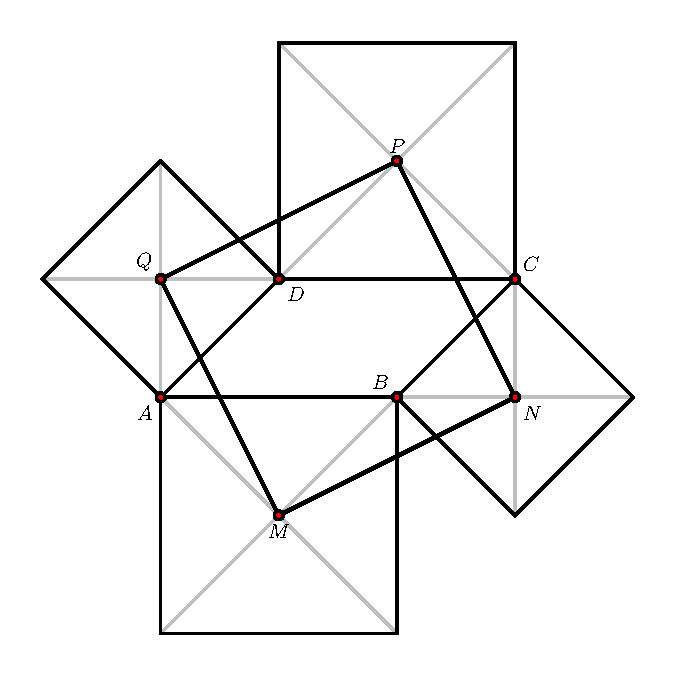
\includegraphics[height=59mm]{img_paralellogramme}}}
  \end{minipage}

  \begin{enumerate}
    \item Déterminer l'affixe de $C$.
    \item Déterminer les affixes des points $M$, $N$, $P$ et $Q$.
    \item Montrer que $MNPQ$ est un carré.
  \end{enumerate}

\end{exo}

\begin{solution}
  \begin{enumerate}
    \item Comme $C = B + \vv{AD}$, l'affixe de $C$ est $1+z$.
    \item Les affixes des points sont $M = \frac{1-i}{2}$, $N = 1+z\frac{1-i}{2}$, $P = z+\frac{1+i}{2}$ et $Q = z\frac{1+i}{2}$.\\
    \emph{Remarque : dans une «bonne» rédaction il va falloir justifier ces résultats.}
    \item Les affixes des vecteurs sont $\vv{MN} = 1+z\frac{1-i}{2} - \frac{1-i}{2} = z\frac{1-i}{2} + \frac{1+i}{2}$, $\vv{QP} = z+\frac{1+i}{2} - z\frac{1+i}{2} = z\frac{1-i}{2} + \frac{1+i}{2}$ et $\vv{MQ} = z\frac{1+i}{2} - \frac{1-i}{2}$. Donc d'une part $\vv{MN} = \vv{QP}$ (donc c'est un parallélogramme), d'autre part comme  $i\left(z\frac{1-i}{2} + \frac{1+i}{2}\right) = z\frac{1+i}{2} - \frac{1-i}{2}$ on a
    que $\vv{MQ}$ est l'image de $\vv{MN}$ par une rotation d'angle $\frac{\pi}{2}$, et donc il s'agit bien d'un carré.
  \end{enumerate}
\end{solution}

\end{document}
